\documentclass{article}

\usepackage{microtype}
\usepackage{graphicx}
\usepackage{booktabs}
\usepackage{amsmath}
\usepackage{amssymb}
\usepackage{hyperref}
\usepackage{enumitem}
\usepackage{tikz}
\usepackage{pgfplots}
\usepackage{placeins}
\usepackage{flafter}

\usetikzlibrary{arrows.meta,positioning,calc,fit,shapes.geometric}
\pgfplotsset{compat=1.18}
\makeatletter
\setlength{\@fptop}{0pt}
\setlength{\@dblfptop}{0pt}
\setlength{\@fpsep}{8pt plus 1pt}
\setlength{\@dblfpsep}{8pt plus 1pt}
\makeatother
\newcommand{\repairkv}{\textsc{RepairKV}}
\newcommand{\bbase}{\ensuremath{B_{\mathrm{base}}}}
\newcommand{\bmatch}{\ensuremath{B_{\mathrm{match}}}}
\newcommand{\spanref}{\ensuremath{\mathrm{SpanRef}\mbox{-}K}}

\usepackage{icml2026}

\icmltitlerunning{Cache Me if You Can: Post-Compression KV Repair}

\begin{document}

\twocolumn[
  \icmltitle{Cache Me if You Can: Post-Compression KV Repair for\\
    Long-Context Agentic LLM Inference}

  \begin{icmlauthorlist}
    \icmlauthor{Andrew Rusli}{equal,harvard}
    \icmlauthor{Shreyan Paliwal}{equal,harvard,opt32}
  \end{icmlauthorlist}
  \icmlaffiliation{equal}{Equal contribution}
  \icmlaffiliation{harvard}{Harvard College, Cambridge, MA, USA}
  \icmlaffiliation{opt32}{Opt32}
  \icmlcorrespondingauthor{Shreyan Paliwal}{shreyanpaliwal@college.harvard.edu}
  \icmlkeywords{resource-adaptive inference, dynamic KV cache compression,
    KV cache repair, between-turn relevance shift, quality-resource tradeoffs}
  \vskip 0.3in
]

\printAffiliationsAndNotice{\icmlEqualContribution}

\begin{abstract}
  As large language models (LLMs) support longer contexts and more capable agentic sessions, what matters in the accumulated context can change with each new query, tool output, test result, or browser observation.
  At the same time, inference still depends on a limited active key-value (KV) cache, and many existing KV-cache compression methods decide which past tokens stay active from the current prefix.
  As a result, tokens that matter in later turns may already have been evicted or compressed away in earlier compression decisions. 
  We study post-compression KV cache repair, a runtime mechanism that restores previously evicted tokens to the active cache.
  \repairkv{} uses the interval between turns to reevaluate which tokens are important from evicted KV rows stored in a slower memory tier, then promotes a small subset before decoding resumes.
  {    Controlled experiments show that \repairkv{}'s restoration of evicted tokens improves retrieval accuracy, with the effect persisting across relevance changes and different initial eviction policies, and a preliminary diagnostic on open-source repositories shows the same pattern; on Qwen2.5-7B-Instruct at 32K context, \repairkv{} achieves 91.0\% retrieval on a four-query needle-in-a-haystack task versus 24.5\% for the matched no-repair baseline at the same active-cache budget, with only 96 promoted tokens.
  }
\end{abstract}
 
% -----------------------------------------------------------------------
\section{Introduction}
% -----------------------------------------------------------------------

Modern language models support context lengths from tens of thousands to
over a million tokens for retrieval-augmented and agentic
workflows~\citep{ruler,longbench,inftybench}, but the KV cache holding
past {token} keys and values grows linearly with sequence length, making it a
primary GPU memory bottleneck {and an increasing runtime cost during decoding. KV-cache compression and offload~\citep{snapkv,streamingllm,h2o,vllm}  manage this cost by deciding which historical state remains active on GPU and which part is evicted or moved to a slower tier.} This decision is usually made with information available at the current turn, and compression is often treated as a one-way operation: evict now, decode later from the retained active set.

This view misses a central feature of multi-turn inference: { new turn signals from } retrieved documents, tool outputs, test failures, or file changes
can make previously low-priority context newly important. {These workflows also create} non-decoding intervals while the
model waits for external results. Together, {the new signal and the pause create an opportunity to repair} the active KV state before the next decode, but {no existing work studies whether an already-compressed cache can be revised in runtime under a matched active-cache budget.}

{This paper studies this gap. Our contributions are:} (1) a matched resumed active-cache-budget protocol for testing whether repair helps without simply keeping more active tokens; (2) \repairkv{}, {an operator conditioned on the next turn's signal that scores evicted KV rows and promotes a small budgeted subset back into the active cache before decoding resumes}; (3) controlled evidence across synthetic relevance shifts, different initial eviction policies, preliminary real-repository diagnostics, and runtime feasibility probes. On Qwen2.5-7B-Instruct at 32K context, \repairkv{} achieves $91.0\%$ retrieval on a four-query needle-in-a-haystack task versus $24.5\%$ for the matched no-repair baseline at the same active-cache budget, with only $96$ promoted tokens.

% -----------------------------------------------------------------------
\section{Related Work}
\label{sec:related}
% -----------------------------------------------------------------------

\subsection{KV-cache compression and eviction}
{KV-cache compression and eviction methods reduce active KV state by retaining a fixed budget of tokens or blocks based on prefix-time, recency, or attention signals~\citep{snapkv,streamingllm,h2o,scissorhands,pyramidkv}}, but this retention decision is usually one-way: rows dropped from the active set cannot re-enter when later turns make them important. This failure mode is observed in recent analyses of instruction and fact degradation under KV compression~\citep{pitfalls}.

\subsection{Query-aware retrieval and sparse attention}
Query-aware methods such as QUEST {emphasize the premise behind repair: token criticality depends on current information need, not only on the prefix that produced the compressed cache~\citep{quest}}. Fine-grained KV retrieval systems use this signal during active decoding to select or fetch query-relevant rows from a retained or indexed KV store~\citep{quest,fier,pariskv,shadowkv}. Attention analyses likewise show that token importance can be query-dependent or recurrent rather than fixed once compressed~\citep{retrieval_heads,lazy_eviction}. {\repairkv{} builds on this query-dependence, but applies it at a different lifecycle point: after compression and before the next decode.}

\begin{figure}[t]
\centering
\resizebox{\linewidth}{!}{%
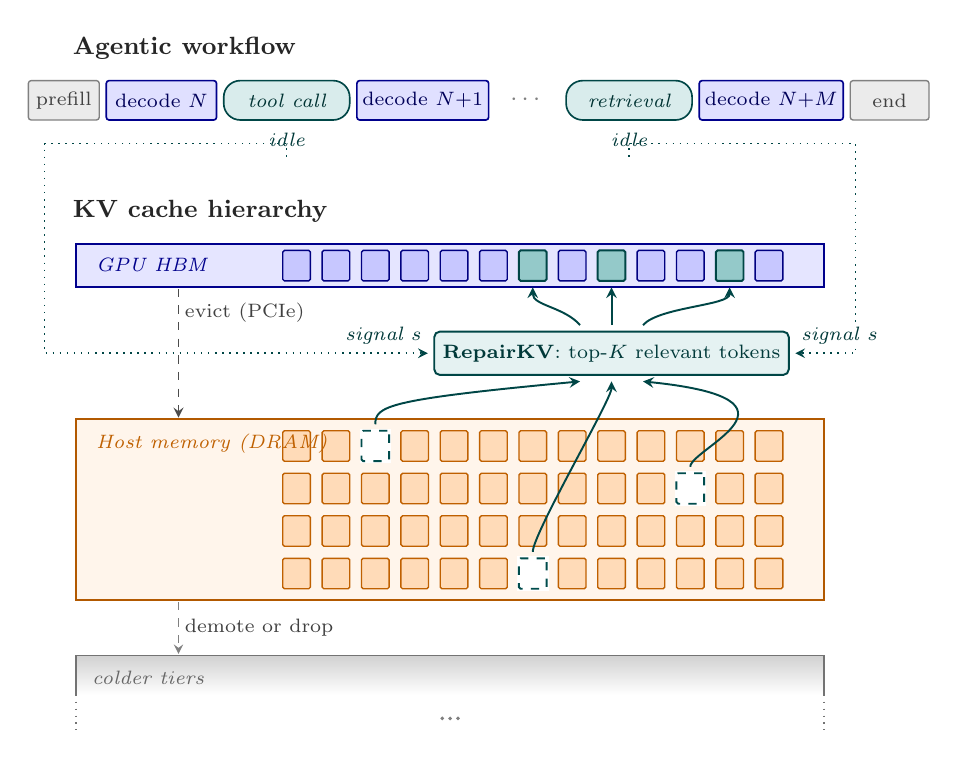
\begin{tikzpicture}[
  >=latex, line width=0.4pt, font=\small,
  active/.style={draw=blue!55!black, fill=blue!10, line width=0.6pt,
                 inner sep=2pt},
  store/.style={draw=orange!70!black, fill=orange!8, line width=0.6pt,
                inner sep=2pt},
  arrlabel/.style={font=\scriptsize, text=black!75, fill=white, inner sep=1pt},
  chip/.style={rounded corners=0.6pt, minimum width=10pt, minimum height=11pt,
               inner sep=0pt, line width=0.5pt},
  gpuchip/.style={chip, draw=blue!50!black, fill=blue!22},
  hostchip/.style={chip, draw=orange!75!black, fill=orange!28},
  promchip/.style={chip, draw=teal!55!black, fill=teal!42, line width=0.7pt},
  ghostchip/.style={chip, draw=teal!60!black, fill=white, dashed, line width=0.7pt},
  evprefill/.style={draw=black!50, fill=black!8, line width=0.5pt,
                    rounded corners=1pt, minimum height=0.50cm,
                    inner sep=2pt, align=center, font=\scriptsize, text=black!75},
  evdecode/.style={draw=blue!55!black, fill=blue!12, line width=0.6pt,
                   rounded corners=1pt, minimum height=0.50cm,
                   inner sep=2pt, align=center, font=\scriptsize, text=blue!35!black},
  evidle/.style={draw=teal!55!black, fill=teal!15, line width=0.6pt,
                 rounded corners=6pt, minimum height=0.50cm,
                 inner sep=2pt, align=center,
                 font=\scriptsize\itshape, text=teal!40!black},
  evictarr/.style={->, line width=0.6pt, draw=black!70, dashed, >=stealth},
  promarr/.style={->, line width=1.2pt, draw=teal!55!black, >=stealth}
]
\def\xL{0.10}

% Section header: Agentic workflow.
\def\labelX{0.55}
\node[font=\bfseries\small, text=black!85, anchor=south west]
     at (\labelX, 6.35) {Agentic workflow};

% Workflow event row.
\def\evY{5.95}
\node[evprefill, minimum width=0.9cm, anchor=west] (evP)  at (\xL,\evY) {prefill};
\node[evdecode,  minimum width=1.4cm, anchor=west, right=2pt of evP]  (evD1) {decode~$N$};
\node[evidle,    minimum width=1.6cm, anchor=west, right=2pt of evD1] (evI1) {tool call};
\node[evdecode,  minimum width=1.6cm, anchor=west, right=2pt of evI1] (evD2) {decode~$N{+}1$};
\node[anchor=west, font=\small, text=black!50, right=4pt of evD2] (evDots) {$\cdots$};
\node[evidle,    minimum width=1.6cm, anchor=west, right=4pt of evDots] (evI2) {retrieval};
\node[evdecode,  minimum width=1.6cm, anchor=west, right=2pt of evI2] (evD3) {decode~$N{+}M$};
\node[evprefill, minimum width=1.0cm, anchor=west, right=2pt of evD3] (evEnd) {end};

% Italic "idle" sub-labels under each pause pill — sources of the dotted signal arrows.
\node[font=\itshape\scriptsize, text=teal!45!black, anchor=north]
     (idleA) at ([yshift=-1pt]evI1.south) {idle};
\node[font=\itshape\scriptsize, text=teal!45!black, anchor=north]
     (idleB) at ([yshift=-1pt]evI2.south) {idle};

% Section header: KV cache hierarchy.
\node[font=\bfseries\small, text=black!85, anchor=south west]
     at (\labelX, 4.275) {KV cache hierarchy};

% Geometry: workflow centered on box midpoint; prefill juts left, end juts right symmetrically.
\def\boxW{9.50}
\pgfmathsetmacro{\boxCx}{(\xL + 10.83)/2}
\pgfmathsetmacro{\boxLeft}{\boxCx - \boxW/2}

% --- Active strip (single row of 13 chips). ---
\def\actY{3.85}
\def\actH{0.55}
\node[active, minimum width=\boxW cm, minimum height=\actH cm, anchor=center]
     (actBox) at (\boxCx, \actY) {};

% 13 chips: 10 blue + 3 teal SCATTERED at cols 7, 9, 12 (at original sequence positions).
\def\actChipStep{0.50}
\pgfmathsetmacro{\actXa}{\boxLeft + 2.80}
\foreach \i in {1,2,3,4,5,6,8,10,11,13}{%
  \pgfmathsetmacro{\xc}{\actXa + (\i-1)*\actChipStep}
  \node[gpuchip] (gpuChip\i) at (\xc, \actY) {};
}
\foreach \i in {7,9,12}{%
  \pgfmathsetmacro{\xc}{\actXa + (\i-1)*\actChipStep}
  \node[promchip] (gpuChip\i) at (\xc, \actY) {};
}
\pgfmathsetmacro{\tealClusterX}{\actXa + 8*\actChipStep}
\node[font=\itshape\scriptsize, text=blue!55!black, anchor=north west]
     at ([xshift=4pt, yshift=-2pt]actBox.north west) {GPU HBM};

% --- Host box (4 rows x 13 cols, columns aligned with GPU active). ---
\def\hostY{0.75}
\def\hostH{2.30}
\node[store, minimum width=\boxW cm, minimum height=\hostH cm, anchor=center]
     (hostBox) at (\boxCx, \hostY) {};

\def\hostRowStep{0.54}
\def\hostColStep{0.50}
\pgfmathsetmacro{\hostXa}{\actXa}
\pgfmathsetmacro{\hostYra}{\hostY + 1.5*\hostRowStep}
\pgfmathsetmacro{\hostYrb}{\hostY + 0.5*\hostRowStep}
\pgfmathsetmacro{\hostYrc}{\hostY - 0.5*\hostRowStep}
\pgfmathsetmacro{\hostYrd}{\hostY - 1.5*\hostRowStep}

\foreach \yr in {\hostYra, \hostYrb, \hostYrc, \hostYrd}{%
  \foreach \i in {1,...,13}{%
    \pgfmathsetmacro{\xc}{\hostXa + (\i-1)*\hostColStep}
    \node[hostchip] at (\xc, \yr) {};
  }
}
% 3 ghost slots showing positions vacated by promotion.
\pgfmathsetmacro{\gxA}{\hostXa + 2*\hostColStep}
\pgfmathsetmacro{\gxB}{\hostXa + 10*\hostColStep}
\pgfmathsetmacro{\gxC}{\hostXa + 6*\hostColStep}
\fill[white] (\gxA - 0.20, \hostYra - 0.22) rectangle (\gxA + 0.20, \hostYra + 0.22);
\fill[white] (\gxB - 0.20, \hostYrb - 0.22) rectangle (\gxB + 0.20, \hostYrb + 0.22);
\fill[white] (\gxC - 0.20, \hostYrd - 0.22) rectangle (\gxC + 0.20, \hostYrd + 0.22);
\node[ghostchip] (ghostA) at (\gxA, \hostYra) {};
\node[ghostchip] (ghostB) at (\gxB, \hostYrb) {};
\node[ghostchip] (ghostC) at (\gxC, \hostYrd) {};

\node[font=\itshape\scriptsize, text=orange!75!black, anchor=north west]
     at ([xshift=4pt, yshift=-2pt]hostBox.north west) {Host memory (DRAM)};

% --- Evict arrow GPU->Host. ---
\pgfmathsetmacro{\evictX}{\boxLeft + 1.30}
\pgfmathsetmacro{\midY}{(\actY - \actH/2 + \hostY + \hostH/2)/2}
\draw[evictarr]
     (\evictX, \actY - \actH/2 - 0.02)
     -- (\evictX, \hostY + \hostH/2 + 0.02);
\node[arrlabel, anchor=west]
     at (\evictX + 0.04, \actY - \actH/2 - 0.32) {evict (PCIe)};

% --- RepairKV operator pill, between Active and Host. ---
\pgfmathsetmacro{\rkvBoxX}{\tealClusterX}
\node[draw=teal!55!black, fill=teal!10, line width=0.7pt, rounded corners=2pt,
      inner sep=3pt, font=\scriptsize, text=teal!45!black, align=center,
      minimum width=2.6cm, minimum height=0.55cm]
     (rkvMid) at (\rkvBoxX, \midY) {\textbf{\repairkv{}}: top-$K$ relevant tokens};

% Three input arrows from host ghost slots up into RepairKV.
\draw[promarr, line width=0.7pt]
     ([yshift=2pt]ghostA.north)
     .. controls ([yshift=0.3cm]ghostA.north) and ([xshift=-0.6cm, yshift=-0.3cm]rkvMid.south west) ..
     ([xshift=-0.4cm, yshift=-2pt]rkvMid.south);
\draw[promarr, line width=0.7pt]
     ([yshift=2pt]ghostB.north)
     .. controls ([yshift=0.3cm]ghostB.north) and ([xshift=0.4cm, yshift=-0.3cm]rkvMid.south east) ..
     ([xshift=0.4cm, yshift=-2pt]rkvMid.south);
\draw[promarr, line width=0.7pt]
     ([yshift=2pt]ghostC.north)
     .. controls ([yshift=0.3cm]ghostC.north) and ([yshift=-0.3cm]rkvMid.south) ..
     ([yshift=-2pt]rkvMid.south);

% Three output arrows from RepairKV up to scattered teal chips at cols 7, 9, 12.
\draw[promarr, line width=0.7pt]
     ([xshift=-0.4cm, yshift=2pt]rkvMid.north)
     .. controls ([xshift=-0.6cm, yshift=0.3cm]rkvMid.north) and ([yshift=-0.3cm]gpuChip7.south) ..
     ([yshift=-2pt]gpuChip7.south);
\draw[promarr, line width=0.7pt]
     ([yshift=2pt]rkvMid.north) -- ([yshift=-2pt]gpuChip9.south);
\draw[promarr, line width=0.7pt]
     ([xshift=0.4cm, yshift=2pt]rkvMid.north)
     .. controls ([xshift=0.6cm, yshift=0.3cm]rkvMid.north) and ([yshift=-0.3cm]gpuChip12.south) ..
     ([yshift=-2pt]gpuChip12.south);

% Two dotted arrows from idle events to RepairKV — carrying signal s.
\pgfmathsetmacro{\detourLX}{\boxLeft - 0.40}
\pgfmathsetmacro{\detourRX}{\boxLeft + \boxW + 0.40}
\draw[->, line width=0.55pt, draw=teal!55!black, dotted, >=stealth]
     (idleA.south) |- (\detourLX, 5.40)
     -- (\detourLX, \midY)
     -- ([xshift=-2pt]rkvMid.west);
\draw[->, line width=0.55pt, draw=teal!55!black, dotted, >=stealth]
     (idleB.south) |- (\detourRX, 5.40)
     -- (\detourRX, \midY)
     -- ([xshift=2pt]rkvMid.east);

% "signal s" labels riding the dotted lines just outside RepairKV.
\node[font=\itshape\scriptsize, text=teal!45!black, anchor=south east,
      fill=white, inner sep=1pt]
     at ([xshift=-3pt, yshift=2pt]rkvMid.west) {signal $s$};
\node[font=\itshape\scriptsize, text=teal!45!black, anchor=south west,
      fill=white, inner sep=1pt]
     at ([xshift=3pt, yshift=2pt]rkvMid.east) {signal $s$};

% --- Colder tiers (faded, open-bottom). ---
\def\coldYtop{-1.10}
\def\coldYbot{-1.60}
\pgfmathsetmacro{\coldL}{\boxLeft}
\pgfmathsetmacro{\coldR}{\boxLeft + \boxW}
\shade[top color=black!18, bottom color=white]
     (\coldL, \coldYbot) rectangle (\coldR, \coldYtop);
\draw[draw=black!55, line width=0.6pt] (\coldL, \coldYtop) -- (\coldR, \coldYtop);
\draw[draw=black!55, line width=0.6pt] (\coldL, \coldYtop) -- (\coldL, \coldYbot);
\draw[draw=black!55, line width=0.6pt] (\coldR, \coldYtop) -- (\coldR, \coldYbot);
\draw[draw=black!55, line width=0.5pt, dotted]
     (\coldL, \coldYbot) -- (\coldL, \coldYbot - 0.45);
\draw[draw=black!55, line width=0.5pt, dotted]
     (\coldR, \coldYbot) -- (\coldR, \coldYbot - 0.45);
\foreach \dx in {-0.10, 0, 0.10}{%
  \fill[black!50] ({\boxCx + \dx}, \coldYbot - 0.30) circle (0.025);
}
\node[font=\itshape\scriptsize, text=black!60, anchor=north west]
     at (\coldL + 0.08, \coldYtop - 0.08) {colder tiers};

% Spill arrow Host -> Cold.
\pgfmathsetmacro{\spillX}{\evictX}
\draw[->, line width=0.5pt, draw=black!50, dashed, >=stealth]
     (\spillX, \hostY - \hostH/2 - 0.02)
     -- (\spillX, \coldYtop + 0.02);
\node[arrlabel, anchor=west]
     at (\spillX + 0.04, {(\hostY - \hostH/2 + \coldYtop)/2}) {demote or drop};
\end{tikzpicture}%
}
\caption{{\repairkv{} system overview. During agent decode pauses (tool calls, retrievals), a selected signal $s$ (such as a new user query, a tool result, retrieved content, or the model's recent generation) is used to rank host KV rows; the top-$K$ are lifted back into GPU HBM at their original sequence positions.}}
\label{fig:pipeline}
\end{figure}

\subsection{Long-context benchmarks}
Long-context benchmarks stress whether models can use information across long inputs, {from ordinary long documents to 100k-token settings}, showing that application-visible context length
does not remove the need for memory-management
mechanisms~\citep{longbench,inftybench,ruler}. {SCBench directly evaluates tasks around the KV-cache lifecycle itself~\citep{scbench}. However, these benchmarks leave open what happens after a compression decision has already removed future-relevant tokens from the active cache.}

\subsection{KV serving and tiering}
Serving systems address the systems side of long-context KV cache management.
PagedAttention/vLLM improves GPU KV allocation and block management
during serving~\citep{vllm}, while prefix-caching systems reduce repeated prefill when requests share or resume prefixes~\citep{lmcache,ttkv}. KV-tiering systems extend this idea across GPU, host memory, storage, and network tiers~\citep{lmcache,ttkv,agentserve}. {Together, these systems determine where KV state lives and when it can be reused, but they do not address the complementary decision of which offloaded rows should re-enter the active cache for the next turn.}

\subsection{Multi-turn LLM serving}
Multi-turn agent workloads pause decoding for external actions such as tool calls, web interaction, repository edits, and tests~\citep{toollm,webarena,swebench,agentbench}. Serving systems make these pauses operationally visible: Continuum schedules multi-turn agent requests around tool-call gaps and KV-cache lifetimes, while AgentServe targets local agent serving under tight GPU memory budgets~\citep{continuum,agentserve}. Pause-aware systems preserve paused-request KV to avoid repeated prefill~\citep{infercept,continuum,cachedattention}. {These same pauses often contain new relevance signals, creating the setting for repair.}

% -----------------------------------------------------------------------
\section{\repairkv{}}
\label{sec:method}
% -----------------------------------------------------------------------

\subsection{Overview}
Each compression step can only choose the active KV set with the information available at that point.
{\repairkv{} treats the resulting compressed state as revisable: when a new turn signal becomes available, the runtime can score offloaded evicted KV rows and promote a small subset before decoding resumes.}
Figure~\ref{fig:pipeline} summarizes this system view.

At the pause boundary, the abstraction has three objects:
\begin{itemize}[leftmargin=1.4em,noitemsep,topsep=2pt]
  \item $C_{\mathrm{base}}$: active evictable KV, with
  $|C_{\mathrm{base}}|=\bbase$ (base active-cache budget);
  \item $W_N$: offloaded evicted KV, hidden from decoding unless promoted; 
  \item $s$: {the pause boundary signal used to score evicted KV,} such as a new user
  query, a tool result, the model's recent generation, or other tokens
  that {indicate upcoming significance.}
\end{itemize}
{The repair map chooses $S_K(s)\subseteq W_N$ with
$|S_K|\le K$, where $K$ is the restore budget}, and resumes from
$C_{\mathrm{repair}}=C_{\mathrm{base}}\cup S_K$ at resumed
active-cache budget $|C_{\mathrm{repair}}|\le \bbase+K$. 

\subsection{Two-turn protocol}
{We isolate multi-turn repair with a protocol for the simplest controlled case: one relevance shift across two turns. A five-turn revisit diagnostic (Figure~\ref{fig:multiturn}) confirms that the effect persists across repeated shifts.}

At turn $N$, the model receives a long distractor document followed by prompt $Q_1$ and generates the response to $Q_1$ from the full uncompressed cache. The runtime then compresses the distractor document KV to a base budget $\bbase$ on GPU and offloads the evicted rows to host memory as $W_N$. The $Q_1$ prompt and the generated response are preserved exactly. During the subsequent idle window, the turn-$(N{+}1)$ prompt $Q_2$ becomes known and is preserved verbatim.

At turn $N{+}1$, the distractor document is not re-presented. \repairkv{} scores the evicted store $W_N$ against the active post-$Q_1$ cache and the $Q_2$ signal, promotes a $K$-budgeted subset $S_K$ back to GPU before $Q_2$ decoding, and the model answers $Q_2$ from $C_{\mathrm{repair}}$.

The primary comparison excludes full-prefill recompute because it reprocesses the long context after $Q_2$ is known, while our comparison asks whether the already-compressed cache can be improved under the same resumed active-cache budget. The controlled prototype evaluates one paused request on one GPU with a single host-memory tier, a prematerialized evicted-KV store, and the full $Q_2$ signal known before resumed decoding.

\subsection{Repair operation}
Intuitively, \repairkv{} {uses the next-turn signal to identify which evicted KV rows should be active before decoding resumes.} Algorithm~\ref{alg:repair} describes the general framework; the prototype is specified by two main choices: {$\textsc{Score}$ and $\textsc{Select}$, with $\mathcal{C}=C_{\mathrm{base}}$ and $\mathcal{W}=W_N$.}
\begin{algorithm}[t]
\caption{General \repairkv{} Execution Framework}
\label{alg:repair}
\begin{algorithmic}[1]
\STATE \textbf{Input:} turn signals $\{s_N\}_{N=1}^T$, 
eviction policy $\mathcal{P}$, base budget $\bbase$, restore
budget $K$.
\STATE \textbf{Initialize:} active cache $\mathcal{C}$,
evicted store $\mathcal{W}\!\gets\!\emptyset$.
\FOR{$N = 1$ to $T$}
  \STATE $\mathrm{ans}_N \gets \textsc{Decode}(\mathcal{C}, s_N)$ \hfill // Decoding
  \STATE $\mathcal{C}, \mathcal{W} \gets \mathcal{P}(\mathcal{C}, \mathcal{W}, \bbase)$ \hfill // Compression
  \STATE obtain $s_{N+1}$ \hfill // Idle window begins
  \FOR{$i \in \mathcal{W}$}
    \STATE $a_i \gets \textsc{Score}(i \mid \mathcal{C}, s_{N+1})$ \hfill // Scoring
  \ENDFOR
  \STATE rank $\mathcal{W}$ by $a_i$ \hfill // Ranking
  \STATE $S_K \gets \textsc{Select}(\mathcal{W}, K)$, $|S_K|\!\le\!K$ \hfill // Selection
  \STATE $\mathcal{C} \gets \mathcal{C}\!\cup\!S_K$;\, $\mathcal{W} \gets \mathcal{W}\!\setminus\!S_K$ \hfill // Repair
\ENDFOR
\end{algorithmic}
\end{algorithm}

For \textsc{Score}, post-RoPE $Q_2$ query tensors
$\{q^{(\ell,h)}_{2,t}\}$ are {scored} against keys in the active and
offloaded sets via
\begin{equation}
  A^{(\ell,h)} = \mathrm{softmax}\!\left(
    \frac{q^{(\ell,h)}_{2,:}\, [K_{C_{\mathrm{base}}},\, K_{W_N}]^{\top}}
         {\sqrt{d_k}}
  \right),
  \label{eq:score-attn}
\end{equation}
restricted to columns in $W_N$, then aggregated as
$a_i = \mathrm{mean}_{\ell, h} \max_t A^{(\ell,h)}_{t,i}$.
Because the softmax normalizes over the active and offloaded keys,
$a_i$ is the attention mass row $i$ would receive given
$C_{\mathrm{base}}$ rather than a raw inner product. Ties break
by the per-token score from the turn-$N$ initial compression, then
by ascending position.

For \textsc{Select}, each top-ranked anchor $i$ is
expanded into a local burst $\{i{-}L,\dots,i{+}R\} \cap (W_N \setminus
S_K)$ under a strict $|S_K| \le K$ budget. The right-biased
$(L, R) = (2, 20)$ {reflects the local structure: high-scoring anchors often occur near queried keys, and answer-bearing value tokens usually follow nearby.} If anchor bursts do not exhaust $K$,
remaining slots backfill from single ranked rows.

The current prototype scores token rows with fixed burst widths. A systems implementation would promote cached blocks or pages.

\subsection{Matched-budget evaluation}
All main claims compare \repairkv{} to a no-repair baseline at the same
resumed active-cache budget. {In both conditions, $Q_2$ decoding sees the same number} of active evictable-context tokens in addition to the
identical preserved $Q_1$ prompt and answer tail. The match is only on active GPU KV: extra offloaded rows, scorer time, and transfer time are not part of the matched budget; they are reported separately as service costs.

{Let $\bmatch$ denote the no-repair condition, which applies the base eviction policy with active evictable-context budget $\bbase+K$. \repairkv{} reaches the same active budget by starting from $\bbase$ retained rows and promoting up to $K$ rows from the host-memory store.

The main restore-budget frontier reports raw answer score. For effect size comparisons, we also report gain over matched no-repair,
\begin{equation}
  \Delta_{\mathrm{repair}} =
  \mathrm{Score}(\mathrm{RepairKV}) - \mathrm{Score}(B_{\mathrm{match}})
\end{equation}
where $\mathrm{Score}$ is the mean fraction of held-out $Q_2$ targets recovered correctly per example over the fixed evaluation set shared across all conditions. Stricter exact-set and precision-sensitive scoring serve as confirmatory checks.}

% -----------------------------------------------------------------------
\section{Experimental Setup}
\label{sec:setup}
% -----------------------------------------------------------------------

\subsection{Benchmark family}
{The main benchmark is a split-query version of multi-query needle-in-a-haystack (MQ-NIAH) derived from RULER~\citep{ruler}. We use this family because it exposes the failure mode repair is meant to address: tokens that are unimportant for the first turn can become critical post-compression.

Each example contains key-value needles inside a long distractor context. The first turn queries one subset of keys, the cache is compressed, and the second turn queries a different subset. This gives a controlled relevance shift with annotated future-relevant spans and a shared turn-$N$ history across conditions.

We evaluate 2Q, 4Q, 6Q, and 8Q variants, which use the same task template but increase the number of queried key-value pairs. For each variant, we pool balanced partitions that avoid a recency shortcut: the keys requested in $Q_2$ are not the needles nearest to the end of the context. Appendix Figure~\ref{fig:app-partition-endpoints} summarizes the exact splits.}

\subsection{Evaluation configuration}
{All main experiments use Qwen2.5-7B-Instruct~\citep{qwen} at 32K rendered context on a single RTX PRO 6000 Blackwell GPU. The initial post-$Q_1$ compression is context-only SnapKV compression~\citep{snapkv}: it is applied only to the evictable document context, while the $Q_1$ prompt and generated $Q_1$ response are preserved exactly.}

Per-task base budgets are calibrated so matched no-repair is neither already near full-cache accuracy nor near zero, leaving room to measure whether repair improves the resumed cache. Unless stated otherwise, the fixed sweep is 
\begin{itemize}[leftmargin=1.4em,noitemsep,topsep=2pt]
    \item compressor: context-only SnapKV with
    $R_{\mathrm{ctx}}=128$ (SnapKV observation-window length);
    \item base budgets: $\bbase=8192$ for 2Q, $\bbase=16384$
  for 4Q, and
    $\bbase=18432$ for 6Q/8Q;
    \item restore budgets: $K=8,16,24,32,48,64,80,96,128$;
    \item replay: one shared full-cache-generated $Q_1$
  response per setting and
    condition.
  \end{itemize}
{This replay removes turn-$N$ generation differences, so the frontier isolates resumed-cache selection quality at turn $N{+}1$. MQ-NIAH-2Q/4Q/6Q use fixed 100-example evaluation sets per partition, while MQ-NIAH-8Q uses 24 examples per partition over five partitions.} Prompt and decode settings are reported in the appendix.

\subsection{Scorers}
For the initial turn-$N$ compression, we score context tokens using the generated $Q_1$ response rather than a generic last-32-token suffix. This makes the post-$Q_1$ compressed cache reflect the actual first turn computation.

For repair, the main quality curves use an exact $Q_2$ scorer. We append $Q_2$ to the compressed active cache, extract the model's post-RoPE $Q_2$ query projections, and score active and offloaded key rows under those projections before selecting evicted rows for promotion. This isolates whether the newly revealed turn signal identifies rows worth restoring.

\subsection{Baselines and references}
We compare the full-cache reference, the base compressed cache before repair, matched no-repair $\bmatch$, Random-$K$ and Oldest-$K$ restore controls, and \repairkv{}. Random-$K$ and Oldest-$K$ promote from the same evicted KV store as \repairkv{} without scoring with $Q_2$, testing whether gains come from query-aware repair or generic reinsertion. 

{The specificity study adds StaleQ-$K$ (score with the previous turn query), WrongQ-$K$ (score with another example's $Q_2$) and Refresh-buffered, which reselects the whole $\bbase+K$ context budget from active and offloaded rows after $Q_2$ is known, without full-prefix recomputation. Refresh-buffered exposes selector headroom rather than acting as a main baseline.}

% -----------------------------------------------------------------------
\section{Results}
\label{sec:results}
% -----------------------------------------------------------------------

\subsection{Matched-budget frontier}
Across MQ-NIAH-2Q/4Q/6Q/8Q, \repairkv{} separates from matched no-repair at moderate to large restore budgets. At $K=96$, \repairkv{} scores $0.910$ on 4Q, $0.989$ on 6Q, and $0.960$ on 8Q, while matched no-repair scores $0.245$, $0.422$, and $0.546$, respectively. Figure~\ref{fig:main-frontier} reports the full raw $Q_2$ score frontier. Random-$K$ and Oldest-$K$ stay near matched no-repair, showing that generic reinsertion from the same evicted KV store does not explain the gains. MQ-NIAH-2Q saturates by $K=80$, while matched no-repair remains near $0.06$. Across all twelve balanced partitions at $K=128$, \repairkv{} beats $\bmatch$ and both content-agnostic controls. {Even the weakest partition-level} gains are $0.585$, $0.387$, and $0.292$ for 4Q, 6Q, and 8Q, respectively. (Appendix Figure~\ref{fig:app-partition-endpoints}).
\begin{figure}[t]
  \centering
  
\includegraphics[width=\columnwidth]{figures/frontier_raw_overlay.pdf}
  \caption{{Raw $Q_2$ score under matched resumed-cache budgets. Solid: \repairkv{}; dotted: matched no-repair. Right labels: query count and $\Delta_{96}$ (gain at $K{=}96$).}}
  \label{fig:main-frontier}
\end{figure}

\subsection{Next-turn signal specificity}
Repair gains depend on using the correct newly revealed signal. At $K=48$, StaleQ-$K$ and WrongQ-$K$ stay near matched no-repair, with gains $0.028$ $[-0.021, 0.083]$ and $0.028$ $[-0.014, 0.069]$, while \repairkv{} reaches $0.326$ $[0.243, 0.410]$. {Thus, the improvement is not explained by scoring with any query-like text; the signal must match the upcoming turn. Refresh-buffered reaches $1.000$, showing that relevant rows remain available for stronger selectors to exploit, motivating an open research direction.}
\begin{table}[!ht]
  \centering
  \setlength{\tabcolsep}{3.5pt}
  \caption{Next-turn signal specificity at $K=48$ on MQ-NIAH-4Q
  ($72$ paired example-partition cases). Stale and donor controls test
  whether any query-like signal suffices; Refresh is a full-budget
  reselector over active and offloaded KV.}
  \label{tab:specificity-control}
  \begin{tabular}{@{}lcc@{}}
    \toprule
    Condition & $Q_2$ score & $\Delta$ vs.\ matched [95\% CI] \\
    \midrule
    Matched no-repair & $0.215$ & -- \\
    StaleQ-$K$ & $0.243$ & $+0.028$ [$-0.021$, $0.083$] \\
    WrongQ-$K$ & $0.243$ & $+0.028$ [$-0.014$, $0.069$] \\
    \repairkv{} & $0.542$ & $+0.326$ [$0.243$, $0.410$] \\
    Refresh-buffered & $1.000$ & $+0.785$ [$0.722$, $0.847$] \\
    \bottomrule
  \end{tabular}
\end{table}

\subsection{Repeated relevance shifts}
The repair effect persists when relevance changes repeatedly. On a fixed five-turn MQ-NIAH-8Q revisit schedule $(K=80$, $n=24$), \repairkv{} gains $0.542$ over matched no-repair on non-initial turns (95\% CI $[0.458,0.620]$). Random-$K$ and Oldest-$K$ gain only $0.010$ and $0.021$, and \repairkv{} remains above StaleQ-$K$, suggesting that repair can track the current turn signal across repeated controlled shifts.
\begin{figure}[tbp]
  \centering
  
\includegraphics[width=\columnwidth]{figures/multiturn_hard_trajectory.pdf}
  \caption{Five-turn relevance-shift diagnostic on MQ-NIAH-8Q
  ($\bbase{=}18{,}432$, $K{=}80$, $n{=}24$). Groups show post-priming exact
  scores at equal active-cache budget. Intervals are bootstrap $95\%$
  CIs for \repairkv{}, and Stale-Q uses the previous-turn query.}
  \label{fig:multiturn}
\end{figure}

\subsection{Eviction-policy sensitivity}
\repairkv{} also improves caches produced by other first-stage eviction policies. On MQ-NIAH-4Q, we replace the primary SnapKV-style compressor with H$_2$O-style accumulated attention retention and a StreamingLLM-style sink-plus-recent rule. In both cases, \repairkv{} improves over each policy's matched no-repair baseline while Random-$K$ and Oldest-$K$ remain near baseline (Figure~\ref{fig:policy-breadth}). Under the StreamingLLM-style policy, for example, \repairkv{} gains $0.431$ at $K=128$. A separate Scissorhands-style persistence stress test also clears the matched-budget protocol (Appendix Table~\ref{tab:app-scissorhands-stress}).
\begin{figure}[t]
  \centering
  
\includegraphics[width=\columnwidth]{figures/policy_breadth_delta.pdf}
  \caption{{Eviction-policy sensitivity on MQ-NIAH-4Q ($n{=}24$, $\bbase{=}16{,}384$). Curves show $Q_2$ gain over each policy's matched no-repair; gray band spans Random-$K$/Oldest-$K$.}}
  \label{fig:policy-breadth}
\end{figure}

\subsection{Real-repository diagnostic}
To test external validity beyond MQ-NIAH, we ran a controlled relevance shift diagnostic on 48 callsite examples from 12 open-source repositories drawn from the SWE-bench pool~\citep{swebench} at fixed commits. Each example loads 32K tokens of line-numbered repository context. The first turn asks about a file unrelated to the answer, encouraging compression to evict the later relevant code. The second turn asks for a target identifier at a callsite.

Between turns, an \emph{event} arrives: a description of the callsite with the target identifier redacted. This event replaces the synthetic $Q_2$ signal used in MQ-NIAH, and all conditions decode the same event and question prompt. {At $K=192$, event-only \repairkv{} improves exact identifier accuracy from $18.8\%$ matched no-repair to $72.9\%$. Non-query controls and ToolFile-$K$ remain near matched (Table~\ref{tab:real-repo-diagnostic}). Thus, the gain comes from using the event as a relevance signal, not from generic reinsertion or simply knowing the file name.} 

Label-assisted references show remaining headroom: File-gated \repairkv{} reaches $83.3\%$, and AnchorWindow-$K$ reaches $89.6\%$. This is a small diagnostic rather than a full benchmark, but it shows some initial evidence that the repair approach improves quality beyond the synthetic MQ-NIAH setting. Appendix Figure~\ref{fig:app-real-repo-diagnostic} gives the full audit.
\begin{table}[!ht]
  \centering
  \setlength{\tabcolsep}{4pt}
  \renewcommand{\arraystretch}{0.95}
  \caption{{Real-repository diagnostic at $K{=}192$ on 48 callsite cases from 12 SWE-bench repositories. Accuracy = exact target-identifier recovery. Non-query = best of Random-$K$/Oldest-$K$/StaleQ-$K$/WrongQ-$K$. AnchorWindow and File-gated are label-assisted (others non-label).}}
  \label{tab:real-repo-diagnostic}
  \small
  \begin{tabular}{@{}lr@{}}
    \toprule
    Condition & Accuracy \\
    \midrule
    Matched no-repair & $18.8\%$ \\
    Best non-query control & $16.7\%$ \\
    ToolFile-$K$ & $18.8\%$ \\
    \repairkv{} & $72.9\%$ \\
    File-gated \repairkv{} & $83.3\%$ \\
    AnchorWindow-$K$ & $89.6\%$ \\
    \bottomrule
  \end{tabular}
\end{table}

\subsection{Runtime}
{We run a separate GPU runtime probe for the repair operation, measuring chunked scan, top-$K$ selection, and KV movement over pinned host-memory BF16 tensors with Qwen-shaped dimensions. At $K=5000$, p95 repair latency is $50.0$\,ms at 32K offloaded candidates, $1.20$\,s at 1M, and $4.64$\,s at 4M (Figure~\ref{fig:runtime-envelope}). These numbers are hardware- and model-dependent: larger KV dimensions increase the constant factor, while newer deployment GPUs may reduce it. The key property is that cost scales linearly with the number of candidate KV rows, which keeps repair in the seconds range even at million-row candidate pools, unlike approaches that recompute or score over full context-query interactions with quadratic cost. {At $K{=}96$ the full repair takes around $110$\,ms (p95) versus $2.13$\,s for full-prefix prefill on our system, even with FlashAttention-2/3 speedups~\citep{flashattn2,flashattn3}; see Appendix~\ref{app:p18-supplement} for selector ablations and time-budgeted query-aware baselines.}

These costs are small relative to many agent and tool-use pauses: OS-level execution, including tool calls and setup, can account for 56--74\% of task latency~\citep{agentcgroup}, and tool calls range from sub-second file/shell operations to multi-second tests or code execution~\citep{continuum}. More broadly, the low repair cost suggests a runtime role beyond using otherwise idle GPU time: repair can be run opportunistically at turn boundaries, tool results, retrieval updates, or other state changes to trade a small amount of memory movement and time for substantially better resumed-cache quality.
\begin{figure}[tbp]
  \centering
  
\includegraphics[width=\columnwidth]{figures/runtime_repair_scaling.pdf}
  \caption{{Runtime-capacity probe. (a) p95 of chunked scan + top-$K$ select + KV move at query length 64, Qwen-shaped pinned host BF16 KV. (b) Stage-wise p95 at $K{=}5000$.}}
  \label{fig:runtime-envelope}
\end{figure}

% -----------------------------------------------------------------------
\section{Conclusion}
\label{sec:conclusion}
% -----------------------------------------------------------------------
\enlargethispage{\baselineskip}
\repairkv{} makes the case for revisable KV compression. Existing compression policies decide which past tokens remain active using the information available at compression time. Our results show that this decision can be usefully revised when a later turn reveals a new relevance signal. Across MQ-NIAH-2Q/4Q/6Q/8Q, repeated relevance shifts, alternative eviction policies, and a small real-repository diagnostic, promoting a small set of relevant evicted rows substantially improves resumed-cache quality under the same active-cache budget.

The broader direction is mutable KV memory for resource-adaptive long-context inference. Repair suggests that runtimes need not treat compression as a one-way loss: they can maintain searchable evicted state, score it when new signals arrive, and use cheap promotion to trade a small amount of memory movement for better response quality. This opens several follow-up directions: stronger $Q_2$-aware selectors, page-level repair policies, scheduler-aware repair at arbitrary turn or tool events, and benchmarks with production-style multi-turn traces, hidden future relevance, and explicit accounting for active-cache, offloaded storage, transfer, and recompute cost.

\section*{Impact Statement}
This paper studies inference-time KV-cache repair for long-context language models. Its intended impact is to reduce GPU memory pressure while improving response quality in long-context and agentic settings where relevance changes between turns. We do not foresee novel ethical risks beyond those already inherent to large language model use.}

% -----------------------------------------------------------------------
\begin{thebibliography}{37}

\bibitem[Abhyankar et~al.(2024)]{infercept}
Abhyankar, R., He, Z., Srivatsa, V., Zhang, H., and Zhang, Y.
\newblock InferCept: Efficient intercept support for augmented large
  language model inference.
\newblock In \emph{Proceedings of the 41st International Conference on
  Machine Learning (ICML)}, 2024.

\bibitem[Bai et~al.(2024)]{longbench}
Bai, Y., Lv, X., Zhang, J., Lyu, H., Tang, J., Huang, Z., Du, Z.,
  Liu, X., Zeng, A., Hou, L., Dong, Y., Tang, J., and Li, J.
\newblock LongBench: A bilingual, multitask benchmark for long context
  understanding.
\newblock In \emph{Proceedings of the 62nd Annual Meeting of the
  Association for Computational Linguistics (ACL)}, 2024.

\bibitem[Chen et~al.(2025)]{pitfalls}
Chen, A., Geh, R., Grover, A., Van den Broeck, G., and Israel, D.
\newblock The pitfalls of KV cache compression.
\newblock \emph{arXiv:2510.00231}, 2025.

\bibitem[Dao(2023)]{flashattn2}
Dao, T.
\newblock FlashAttention-2: Faster attention with better parallelism and
  work partitioning.
\newblock \emph{arXiv:2307.08691}, 2023.

\bibitem[d-Matrix(2025)]{dmatrix2025}
d-Matrix.
\newblock Corsair: In-memory computing for AI inference.
\newblock Hot Chips, 2025.

\bibitem[Dzikanyanga et~al.(2026)]{ttkv}
Dzikanyanga, G., Yang, W., Huang, H., Wu, D., Wang, S., Xia, W., and
  K~C, S.
\newblock TTKV: Temporal-tiered KV cache for long-context LLM inference.
\newblock \emph{arXiv:2604.19769}, 2026.

\bibitem[Gao et~al.(2024)]{cachedattention}
Gao, B., He, Z., Sharma, P., Kang, Q., Jevdjic, D., Zhao, J., and
  Zuo, P.
\newblock Cost-efficient large language model serving for multi-turn
  conversations with CachedAttention.
\newblock In \emph{Proceedings of the 2024 USENIX Annual Technical
  Conference (USENIX ATC)}, 2024.

\bibitem[Hsieh et~al.(2024)]{ruler}
Hsieh, C.-Y., Sun, S., Kriman, S., Acharya, S., Rekesh, D., Jia, F.,
  Zhang, Y., and Ginsburg, B.
\newblock RULER: What's the real context window size of your LLM.
\newblock In \emph{Conference on Language Modeling (COLM)}, 2024.

\bibitem[Jimenez et~al.(2024)]{swebench}
Jimenez, C. E., Yang, J., Wettig, A., Yao, S., Pei, K., Press, O.,
  and Narasimhan, K.
\newblock SWE-bench: Can language models resolve real-world GitHub
  issues.
\newblock In \emph{International Conference on Learning
  Representations (ICLR)}, 2024.

\bibitem[Kim et~al.(2025)]{cxlkv2025}
Kim, D., Lee, M., Kim, J., Kwon, H., Jeong, H., Park, S.-S., Yoon, M.,
  Roh, S.-D., Kwon, Y., So, J., and Choi, J.
\newblock Scalable processing-near-memory for 1M-token LLM inference: CXL-enabled KV-cache management beyond GPU limits.
\newblock \emph{arXiv:2511.00321}, 2025.

\bibitem[Kwon et~al.(2023)]{vllm}
Kwon, W., Li, Z., Zhuang, S., Sheng, Y., Zheng, L., Yu, C. H.,
  Gonzalez, J. E., Zhang, H., and Stoica, I.
\newblock Efficient memory management for large language model serving
  with PagedAttention.
\newblock In \emph{Proceedings of the 29th ACM Symposium on Operating
  Systems Principles (SOSP)}, 2023.

\bibitem[Li et~al.(2026)]{continuum}
Li, H., Mang, Q., He, R., Zhang, Q., Mao, H., Chen, X., Zhou, H.,
  Cheung, A., Gonzalez, J., and Stoica, I.
\newblock Continuum: Efficient and robust multi-turn LLM agent
  scheduling with KV cache time-to-live.
\newblock \emph{arXiv:2511.02230}, 2026.

\bibitem[Li et~al.(2024a)]{snapkv}
Li, Y., Huang, Y., Yang, B., Venkitesh, B., Locatelli, A., Ye, H.,
  Cai, T., Lewis, P., and Chen, D.
\newblock SnapKV: LLM knows what you are looking for before generation.
\newblock \emph{arXiv:2404.14469}, 2024.

\bibitem[Li et~al.(2025)]{scbench}
Li, Y., Jiang, H., Wu, Q., Luo, X., Ahn, S., Zhang, C., Abdi, A. H.,
  Li, D., Gao, J., Yang, Y., and Qiu, L.
\newblock SCBench: A KV cache-centric analysis of long-context methods.
\newblock In \emph{International Conference on Learning Representations
  (ICLR)}, 2025.

\bibitem[Li et~al.(2024b)]{pyramidkv}
Li, Z., Yang, Y., Zhang, Y., and Liu, Z.
\newblock PyramidKV: Dynamic KV cache compression based on pyramidal
  information funneling.
\newblock \emph{arXiv:2406.02069}, 2024.

\bibitem[Liu and Yu(2025)]{cxlspeckv2025}
Liu, D. and Yu, Y.
\newblock CXL-SpecKV: A disaggregated FPGA speculative KV-cache for datacenter LLM serving.
\newblock \emph{arXiv:2512.11920}, 2025.

\bibitem[Liu et~al.(2024)]{agentbench}
Liu, X., Yu, H., Zhang, H., Xu, Y., Lei, X., Lai, H., Gu, Y.,
  Ding, H., Men, K., Yang, K., Zhang, S., Deng, X., and others.
\newblock AgentBench: Evaluating LLMs as agents.
\newblock In \emph{International Conference on Learning
  Representations (ICLR)}, 2024.

\bibitem[Liu et~al.(2025)]{lmcache}
Liu, Y., Cheng, Y., Yao, J., An, Y., Chen, X., Feng, S., Huang, Y.,
  Shen, S., Zhang, R., Du, K., and Jiang, J.
\newblock LMCache: An efficient KV cache layer for enterprise-scale LLM
  inference.
\newblock \emph{arXiv:2510.09665}, 2025.

\bibitem[Liu et~al.(2023)]{scissorhands}
Liu, Z., Desai, A., Liao, F., Wang, W., Xie, V., Xu, Z.,
  Kyrillidis, A., and Shrivastava, A.
\newblock Scissorhands: Exploiting the persistence of importance
  hypothesis for LLM KV cache compression at test time.
\newblock In \emph{Advances in Neural Information Processing Systems
  (NeurIPS)}, 2023.

\bibitem[NVIDIA(2026)]{icmsp2026}
NVIDIA.
\newblock NVIDIA BlueField-4 powers new class of AI-native storage infrastructure for the next frontier of AI.
\newblock NVIDIA Newsroom, January 2026.
  Announces the Inference Context Memory Storage Platform (ICMSP) at CES 2026.

\bibitem[Qi et~al.(2026)]{pariskv}
Qi, Y., Chen, X., Jiang, H., Wang, Q., Peng, B., and Palpanas, T.
\newblock ParisKV: Fast and drift-robust KV-cache retrieval for
  long-context LLMs.
\newblock \emph{arXiv:2602.07721}, 2026.

\bibitem[Qin et~al.(2024)]{toollm}
Qin, Y., Liang, S., Ye, Y., Zhu, K., Yan, L., Lu, Y., Lin, Y.,
  Cong, X., Tang, X., Qian, B., Zhao, S., Hong, L., and others.
\newblock ToolLLM: Facilitating large language models to master
  16000+ real-world APIs.
\newblock In \emph{International Conference on Learning
  Representations (ICLR)}, 2024.

\bibitem[Qwen(2024)]{qwen}
Qwen Team.
\newblock Qwen2.5 technical report.
\newblock \emph{arXiv:2412.15115}, 2024.

\bibitem[SambaNova(2024)]{sambanova2024}
SambaNova Systems.
\newblock SN40L reconfigurable dataflow unit, 2024.

\bibitem[Shah et~al.(2024)]{flashattn3}
Shah, J., Bikshandi, G., Zhang, Y., Thakkar, V., Ramani, P., and Dao, T.
\newblock FlashAttention-3: Fast and accurate attention with asynchrony
  and low-precision.
\newblock In \emph{Advances in Neural Information Processing Systems
  (NeurIPS)}, 2024.

\bibitem[Sun et~al.(2025)]{shadowkv}
Sun, H., Chang, L.-W., Bao, W., Zheng, S., Zheng, N., Liu, X., Dong,
  H., Chi, Y., and Chen, B.
\newblock ShadowKV: KV cache in shadows for high-throughput long-context
  LLM inference.
\newblock \emph{arXiv:2410.21465}, 2025.

\bibitem[Tang et~al.(2024)]{quest}
Tang, J., Zhao, Y., Zhu, K., Xiao, G., Kasikci, B., and Han, S.
\newblock QUEST: Query-aware sparsity for efficient long-context LLM
  inference.
\newblock In \emph{Proceedings of the 41st International Conference on
  Machine Learning (ICML)}, 2024.

\bibitem[Wang et~al.(2025)]{fier}
Wang, D., Liu, Z., Wang, S., Ren, Y., Deng, J., Hu, J., Chen, T., and
  Yang, H.
\newblock FIER: Fine-grained and efficient KV cache retrieval for
  long-context LLM inference.
\newblock In \emph{Proceedings of the Conference on Empirical Methods in
  Natural Language Processing (EMNLP)}, 2025.

\bibitem[Wu et~al.(2024)]{retrieval_heads}
Wu, W., Wang, Y., Xiao, G., Peng, H., and Fu, Y.
\newblock Retrieval heads mechanistically explain long-context factuality.
\newblock \emph{arXiv:2404.15574}, 2024.

\bibitem[Xiao et~al.(2024)]{streamingllm}
Xiao, G., Tang, Y., Zuo, J., Guo, J., Yang, S., Tang, H., Fu, Y.,
  and Han, S.
\newblock Efficient streaming language models with attention sinks.
\newblock In \emph{International Conference on Learning Representations
  (ICLR)}, 2024.

\bibitem[Yoon et~al.(2025)]{tract2025}
Yoon, D., Min, Y., Kim, H., Noh, S.~H., and Kim, J.
\newblock TraCT: Disaggregated LLM serving with CXL shared memory KV cache at rack-scale.
\newblock \emph{arXiv:2512.18194}, 2025.

\bibitem[Zhang et~al.(2025)]{lazy_eviction}
Zhang, H., Zhang, H., Ma, X., Zhang, J., and Guo, S.
\newblock LazyEviction: Lagged KV eviction with attention pattern
  observation for efficient long reasoning.
\newblock \emph{arXiv:2506.15969}, 2025.

\bibitem[Zhang et~al.(2024)]{inftybench}
Zhang, X., Chen, Y., Hu, S., Xu, Z., Chen, J., Hao, M. K., Han, X.,
  Thai, Z. L., Wang, S., Liu, Z., and Sun, M.
\newblock $\infty$Bench: Extending long context evaluation beyond 100K
  tokens.
\newblock In \emph{Proceedings of the 62nd Annual Meeting of the
  Association for Computational Linguistics (ACL)}, 2024.

\bibitem[Zhang et~al.(2026)]{agentserve}
Zhang, Y., Yan, Y., Yang, N., and Yuan, D.
\newblock AgentServe: Algorithm-system co-design for efficient agentic
  AI serving on a consumer-grade GPU.
\newblock \emph{arXiv:2603.10342}, 2026.

\bibitem[Zhang et~al.(2023)]{h2o}
Zhang, Z., Sheng, Y., Zhou, T., Chen, T., Zheng, L., Cai, R., Song, Z.,
  Tian, Y., R{\'e}, C., Barrett, C., Wang, Z., and Chen, B.
\newblock H$_2$O: Heavy-hitter oracle for efficient generative inference
  of large language models.
\newblock In \emph{Advances in Neural Information Processing Systems
  (NeurIPS)}, 2023.

\bibitem[Zheng et~al.(2026)]{agentcgroup}
Zheng, Y., Fan, J., Fu, Q., Yang, Y., Zhang, W., and Quinn, A.
\newblock AgentCgroup: Understanding and controlling OS resources of AI
  agents.
\newblock \emph{arXiv:2602.09345}, 2026.

\bibitem[Zhou et~al.(2024)]{webarena}
Zhou, S., Xu, F. F., Zhu, H., Zhou, X., Lo, R., Sridhar, A.,
  Cheng, X., Ou, T., Bisk, Y., Fried, D., Alon, U., and Neubig, G.
\newblock WebArena: A realistic web environment for building autonomous
  agents.
\newblock In \emph{International Conference on Learning
  Representations (ICLR)}, 2024.

\end{thebibliography}

\clearpage
\appendix
\raggedbottom

\section{\texorpdfstring{{Outlook and open directions}}{Outlook and open directions}}
\label{app:outlook}

{We share this prototype as preliminary evidence that compressed KV state can be usefully revised at a turn boundary.
The patterns we observe across matched active-cache budgets, eviction-policy variations, repeated relevance shifts, and a small real-repository diagnostic suggest a mechanism worth deeper study.
We propose several extensions as natural next steps.

\paragraph{Scale and coverage.}
With more compute, we plan to run the matched-budget protocol on additional instruct-tuned families (Llama, Mistral), at larger model scale (70B-class), and at longer contexts (64K, 128K, 256K), where eviction errors compound and the room for repair grows.

\paragraph{Stronger benchmarks.}
SCBench and full SWE-bench resolution are potential short-term next steps.
The ideal benchmark would be closer to production multi-turn agent traces with real tool calls.

\paragraph{Stronger comparisons.}
Running query-aware retrieval methods (e.g., QUEST, ShadowKV) as repair operators under the matched active-cache-budget protocol would isolate selector quality from architectural commitments, alongside end-to-end serving evaluations under realistic deployment baselines.

The mechanism also fits naturally into the multi-tier KV systems that have become a frontier of LLM serving.
NVIDIA's ICMSP makes NVMe-resident KV part of the context address space~\citep{icmsp2026}, CXL-based KV systems push the warm tier off-package with coherent host-side access~\citep{cxlkv2025,tract2025,cxlspeckv2025}, and inference accelerators are exposing tiered memory architectures~\citep{dmatrix2025,sambanova2024}.
The open runtime question across these stacks, namely which slow-tier rows to promote back into the active tier under a budget and on what signal, is the question this mechanism is designed to address.
We see revisable compressed KV as a research primitive worth broader investigation.
}

\section{Additional Evaluation Details}
\label{app:evaluation-details}

\paragraph{Protocol details.}
Concise split prompts request values only, comma-separated, with a short
answer prefix and fixed decode budgets of 24 tokens for MQ-NIAH-4Q,
48 tokens for MQ-NIAH-6Q, and 64 tokens for MQ-NIAH-8Q.
Generation is deterministic greedy decoding with no sampling.
The main examples use dataset seed offset 0.
Random-$K$ uses a
deterministic example- and $K$-dependent seed.
Bootstrap intervals are percentile intervals over paired
example-partition rows with fixed seeds.
Main Qwen runs use BF16 weights on one RTX PRO 6000 Blackwell GPU with
Python 3.12.3, PyTorch 2.10.0+cu128, and Transformers 5.2.0.
The exact-Q$_2$ attention-query selector appends $Q_2$ to
the compressed active cache, extracts the model's post-RoPE query
projections for the $Q_2$ prompt tokens, and scores active and offloaded
key rows under those projections before selecting evicted rows for
promotion. This selector is distinct from decode-time answer-token
attention and from the final answer metric. The $Q_2$-appended-state proxy
appends $Q_2$ to the compressed cache and uses the appended cache rows as
a second Q$_2$-conditioned scoring signal.

\paragraph{Span-group diagnostic.}
\spanref{} starts from the same $B$ state and offloaded evicted-KV store
as \repairkv{}.
It enumerates the small family of annotated $Q_2$ answer-span-group
subsets, one key/value span group per requested needle, evaluates each
subset once under actual $Q_2$ generation, and chooses the
highest-scoring subset with total cost at most $K$.
It is exact over this benchmark-specific span-group family, but not over
all arbitrary token subsets or possible final generations.
Because the selected span-group subset may use fewer than $K$ rows, a
repair selector can occasionally score higher at low budgets by spending
the full budget on useful local neighborhoods around future-relevant
spans. Thus \spanref{} is a diagnostic span-group reference, not a
ceiling. 

\paragraph{Partition choices.}
For MQ-NIAH-4Q, the pooled panel uses
$14{\rightarrow}23$, $24{\rightarrow}13$, and
$34{\rightarrow}12$.
These are the balanced $2|2$ partitions whose $Q_2$ side excludes the
tail-anchored fourth needle.
For MQ-NIAH-6Q, the pooled panel uses
$156{\rightarrow}234$, $256{\rightarrow}134$,
$356{\rightarrow}124$, and $456{\rightarrow}123$, so the second turn
excludes the two latest needles.
For MQ-NIAH-8Q, the pooled panel uses
$5678{\rightarrow}1234$, $1678{\rightarrow}2345$,
$2678{\rightarrow}1345$, $3678{\rightarrow}1245$, and
$4678{\rightarrow}1235$, again excluding the two latest needles from the
second turn.
Within-turn order is not treated as a separate condition because the
prompt asks for comma-separated values only and scoring checks whether
each requested value is recovered.

\paragraph{Scissorhands-style persistence stress test.}
Table~\ref{tab:app-scissorhands-stress} repeats the MQ-NIAH-6Q
matched-budget protocol after replacing the initial SnapKV-style eviction policy with a
one-shot persistence policy inspired by Scissorhands.
The test asks whether repair still works when the compressed active cache
is chosen by past attention persistence in place of the primary eviction
policy.
Canonical online per-head Scissorhands reproduction remains future work.

\begin{table}[H]
  \centering
  \caption{Scissorhands-style persistence stress test on
  MQ-NIAH-6Q ($\bbase{=}18{,}432$, $n{=}24$). Values are exact scores;
  full-cache reference is $0.990$ for all $K$. Best ctrl.\ is the stronger
  of Random-$K$ and Oldest-$K$; CI is the paired bootstrap $95\%$
  interval for \repairkv{}$-\bmatch$.}
  \label{tab:app-scissorhands-stress}
  \small
  \setlength{\tabcolsep}{3.5pt}
  \begin{tabular}{rrrrr}
    \toprule
    $K$ & $\bmatch$ & Ctrl. & \repairkv{} & CI \\
    \midrule
    48 & 0.365 & 0.382 & 0.712 & [0.292, 0.403] \\
    64 & 0.365 & 0.382 & 0.795 & [0.378, 0.490] \\
    80 & 0.378 & 0.385 & 0.934 & [0.503, 0.604] \\
    96 & 0.375 & 0.382 & 0.993 & [0.566, 0.670] \\
    128 & 0.368 & 0.378 & 0.990 & [0.573, 0.674] \\
    \bottomrule
  \end{tabular}
\end{table}

\section{\texorpdfstring{{Additional Analysis and Discussion}}{Additional Analysis and Discussion}}
\label{app:additional-discussion}

\paragraph{Tiered-cache scaling.}
Our current repair mechanism creates a two-level cache-budget problem because the main curves match
the resumed active GPU KV budget while tracking total host-plus-device
storage separately.
A strict device-resident policy chooses the active-cache budget, while a
looser off-device policy decides which evicted rows remain searchable,
compressed, summarized, or recomputable.
In the Qwen-shaped accounting
above, 4M searchable rows already imply about 240\,GB before metadata.
Thus \repairkv{} supports the middle operation in a tiered hierarchy:
turn-conditioned promotion from host memory during an idle window.
This is a hardware-facing implication and hardware measurement remains
future work.

\paragraph{Idle-window repair interface.}
A practical implementation would expose a host-memory index over evicted KV
units, a time-budgeted selector conditioned on the next-turn signal,
asynchronous promotion into the active cache, and fallbacks to no-repair or
full recompute.

\paragraph{Preliminary nonlinear variable-tracking diagnostic.}
\label{app:vt8hop-div2}

As another direction we began to explore, we also tested a modified RULER
variable-tracking task that makes the dependency structure less linear than the
standard 4-hop chain. The diagnostic uses an 8-hop permuted chain with two
distractor divergences: some assignments introduce branches that are not used by
the final answer, so the model must recover the relevant path through a small
information graph rather than follow a tail-friendly linear sequence. In
32K-context Qwen2.5-7B-Instruct runs, SnapKV compression degraded this task
sharply even at moderate retained-cache budgets. Preliminary repair runs
recovered substantial accuracy from the same compressed states using small
restore fractions. These results are not part of the main evidence, but they
motivate a broader benchmark for nonlinear and conflicting relevance patterns,
where eviction policies may fail even when standard long-context tasks appear
solved. Turning this observation into a robust benchmark is a natural next step
for testing when compression and repair need to operate together.

\paragraph{Future benchmark axes.}
Future benchmarks should vary the number, timing, and conflict structure
of new-turn constraints.
The 2Q and 8Q breadth checks suggest that easy regimes can saturate while
stricter multi-query turns expose how quickly eviction failures
accumulate.
The five-turn diagnostic strengthens the dynamic-workflow evidence, but
it remains synthetic.
Broader task families should keep the same
matched-budget controls while adding real tool traces and stronger
selector families.

\begingroup\section{\texorpdfstring{{Time-Matched Selector Ablations}}{Time-Matched Selector Ablations}}
\label{app:p18-supplement}

\paragraph{Time-budgeted baselines.} Two additional baselines extend the protocol of Section~\ref{sec:setup}, both subject to a wall-clock budget matched to \repairkv{}'s measured per-pause repair time. \textbf{Refresh-$K$-budgeted} is the Refresh-buffered baseline of Section~\ref{sec:setup} with this wall-clock budget applied: when the budget runs out, it stops scoring further evicted positions. \textbf{PageSummary-Quest-inspired} pre-computes per-chunk summary keys (max over each chunk) at compression time, ranks chunks by a cheap inner product against $Q_2$, and within the same wall-clock budget visits top-ranked chunks using the same per-position scorer. Both methods choose from the same evicted store as \repairkv{} and are matched on resumed active-cache rows ($\bbase{+}K$); only their off-budget service costs (scoring time, transfer, projection) differ. All numbers in this supplement come from a smaller paired $n{=}36$ MQ-NIAH-4Q slice, run separately to keep the wall-clock-budgeted baselines tractable; small differences from the $n{=}300$ headline numbers in Section~\ref{sec:results} (e.g., $\bmatch{=}0.208$ here vs.\ $0.245$ there) reflect this resampled slice rather than a protocol change.

\paragraph{Wall-clock-matched K-sweep.} On MQ-NIAH-4Q at a $150$\,ms absolute scoring budget across $K\in\{32,64,96,128\}$ (Qwen2.5-7B-Instruct, $\bbase{=}16{,}384$, $n{=}36$ paired observations per $K$), the budget runs out before Refresh-$K$-budgeted finishes scoring on all $36/36$ examples, scoring approximately $4{,}000$ of $32{,}768$ evicted positions per call. \repairkv{} dominates at $K\geq 64$, reaching $0.917$ at $K{=}96$ against $0.472$ for Refresh-$K$-budgeted and $0.194$ for PageSummary-Quest-inspired (matched no-repair $\bmatch{=}0.208$). At $K{=}128$ under the same budget, \repairkv{} saturates at $1.000$ while the two time-budgeted baselines remain near $0.5$ and $0.2$.

\paragraph{Per-position scoring vs.\ burst-expansion contributions.} The gains decompose into two contributions at $K{=}96$ on Qwen. Promoting only the top-scoring evicted positions, without the burst-expansion step of Section~\ref{sec:method}, reaches $0.653$ and exceeds PageSummary-Quest-inspired by $\Delta_\text{score}{=}{+}0.459$. This isolates the lift from per-position scoring relative to the cheaper per-chunk-summary scorer. Adding burst expansion lifts \repairkv{} to $0.917$, an additional $\Delta_\text{burst}{=}{+}0.264$. Per-position scoring contributes the larger share.
\endgroup

\section{\texorpdfstring{{Additional Experiments}}{Additional Experiments}}
\label{app:supplementary-figures}

The supplementary figures probe external validity,
query-count and operating-regime breadth, partition consistency, runtime
capacity, and appendix selector diagnostics.
\FloatBarrier

\IfFileExists{figures/real_repo_repair_diagnostic.pdf}{%
\begin{figure}[!ht]
  \centering
  
\includegraphics[width=\columnwidth]{figures/real_repo_repair_diagnostic.pdf}
  \caption{Controlled real-repository relevance-shift diagnostic over
  $48$ callsite examples from $12$ repositories drawn from the SWE-bench
  repository pool at pinned commits. Repair sees only the event cue. All
  conditions decode the same event-plus-question prompt. Left: exact
  identifier accuracy at $K=96$ and $K=192$. Right: $K=192$ \repairkv{}
  gain over matched no-repair after removing cue-only or answer-retention
  rows. ToolFile-$K$ is file-name-assisted with oldest-row backfill.
  File-gated \repairkv{} restricts candidates to the event-named file before
  applying the event-only scorer. Lexical is an answer-sanitized diagnostic
  outside the deployable-selector comparison.
  AnchorWindow-$K$ is a label-assisted locality reference outside the
  deployable-baseline and end-to-end issue-resolution comparisons.}
  \label{fig:app-real-repo-diagnostic}
\end{figure}
}{}

\IfFileExists{figures/query_count_breadth.pdf}{%
\begin{figure}[!ht]
  \centering
  
\includegraphics[width=\columnwidth]{figures/query_count_breadth.pdf}
  \caption{Query-count breadth: cells show \repairkv{} score gain over
  matched no-repair for $K=48$ and $K=96$ across 2-, 3-, 4-, 6-, and
  8-question split-query variants.}
  \label{fig:app-query-count-breadth}
\end{figure}
}{}

\IfFileExists{figures/operating_regime_heatmap.pdf}{%
\begin{figure}[!ht]
  \centering
  
\includegraphics[width=\columnwidth]{figures/operating_regime_heatmap.pdf}
  \caption{Operating regime: cells show the fraction of available
  \spanref{} diagnostic gain recovered by \repairkv{}, clipped to $[0,1]$,
  for MQ-NIAH-4Q/6Q. Saturated cells with little matched-to-\spanref{}
  gap should not be read as upper-bound statements.}
  \label{fig:app-operating-regime}
\end{figure}
}{}

\IfFileExists{figures/partition_endpoint_dotplot.pdf}{%
\begin{figure}[!ht]
  \centering
  
\includegraphics[width=\columnwidth]{figures/partition_endpoint_dotplot.pdf}
  \caption{Per-partition endpoint scores at $K=128$ on the final exact
  evaluations. Gray segments show the change from matched
  no-repair to \repairkv{}, orange points show the benchmark-metadata
  \spanref{} diagnostic, and labels report the \repairkv{} difference over
  matched no-repair.}
  \label{fig:app-partition-endpoints}
\end{figure}
}{}

\IfFileExists{figures/repair_selection_diagnostic.pdf}{%
\begin{figure}[!ht]
  \centering
  
\includegraphics[width=\columnwidth]{figures/repair_selection_diagnostic.pdf}
  \caption{Mechanism diagnostic for the final exact MQ-NIAH evaluations.
  Curves show overlap between promoted tokens and annotated $Q_2$ answer
  spans. Content-agnostic promotions stay near baseline while \repairkv{}
  increasingly covers future-relevant spans.}
  \label{fig:selection-diagnostic}
\end{figure}
}{}

\IfFileExists{figures/runtime_capacity_curve.pdf}{%
\begin{figure}[!ht]
  \centering
  
\includegraphics[width=\columnwidth]{figures/runtime_capacity_curve.pdf}
  \caption{Move-and-inject capacity: synthetic move-and-inject capacity
  for Qwen-shaped BF16 KV on the evaluation GPU, separate from the
  Figure~\ref{fig:runtime-envelope} scan/select envelope. Measurements
  use pinned host-memory promoted blocks and report p95 latency as $K$
  or active cache size grows.}
  \label{fig:app-runtime-capacity}
\end{figure}
}{}

\IfFileExists{figures/proxy_controlled_frontier.pdf}{%
\begin{figure}[!ht]
  \centering
  
\includegraphics[width=\columnwidth]{figures/proxy_controlled_frontier.pdf}
  \caption{Proxy-selector diagnostic on MQ-NIAH-4Q/6Q ($100$ examples
  per split). At $K=96$, content-agnostic promotions stay within
  $0.010$/$0.004$ of matched no-repair while proxy \repairkv{} remains
  well above matched.}
  \label{fig:app-proxy-controlled}
\end{figure}
}{}

\end{document}
